\section{Function Approximation}
Everything from DP through Q-learning assumed we could afford one table cell per state (or state-action pair). That assumption dies the moment states are continuous (robot joint angles, pixel images) or just combinatorially large (Backgammon has $\sim 10^20$ states) -- there isn't enough memory to store the table, let alone enough experience to fill every cell. Function approximation trades exactness for compactness: instead of memorizing a value per state, we learn a function with far fewer parameters than there are states, and rely on generalization to states we've never visited.

\begin{align*}
    \hat{v}(s,\mathbf{w}) &\approx v_\pi(s) \\
    \text{or }\hat{q}(s, a, \mathbf{w}) &\approx q_\pi(s,a)
\end{align*}

Where $\mathbf{w} \in \mathbb{R}^d$ (with $d \ll \lvert \mathcal{S}\rvert$) represents a \emph{weight vector} that will approximate the value function. This way we can fit a function for each state we will be visiting while also being able to generalize the states which have yet to be seen by querying our function approximator in those states.

Now a question arises: \emph{which} function approximator is to be chosen for RL tasks? From now on we will only consider \textbf{differentiable} function approximators, e.g.:
\begin{itemize}
    \item Linear combinations of features
    \item Neural Networks
    \item \dots
\end{itemize}

The main difference of RL when compared to standard supervised learning is that in practice we end up with a non-stationary (always changing), non-iid (e.g. where I am now is highly correlated to where I will be at the next step) sequence of value functions we're trying to estimate.

\subsection{Incremental Methods}\label{sec:incremental-methods}
\subsubsection{Gradient Descent}
We now develop in detail one class of learning methods for function approximation in value prediction, those based on stochastic gradient descent (SGD). SGD methods are among the most widely used of all function approximation methods and are particularly well suited to online reinforcement learning.

Let $J(\mathbf{w})$ be a differentiable function with parameter vector $\mathbf{w}$. We define the gradient of $J(\mathbf{w})$ with respect to $\mathbf{w}$ as:

\[
\nabla_{\mathbf{w}} J(\mathbf{w}) = 
\begin{pmatrix}
\frac{\partial J(\mathbf{w})}{\partial \mathbf{w}_1} \\
\vdots \\
\frac{\partial J(\mathbf{w})}{\partial \mathbf{w}_n}
\end{pmatrix}
\]

The goal now is to find the local minimum of $J(\mathbf{w})$ and move the parameter $\mathbf{w}$ in the direction of the negative gradient:
\[
    \Delta \mathbf{w} = - \frac{1}{2} \alpha \nabla_{\mathbf{w}} J(\mathbf{w})
\]

With $\alpha$ being the step-size parameter.

Let's now imagine that we have an oracle that tells us the correct value of the value function $v_\pi$; if we had this we could just minimize the MSE between the approximate value and the true function value:

\[
    J(\mathbf{w}) = \mathbb{E}_\pi \left[ (v_\pi(s) - \hat{v}(s,\mathbf{w}))^2 \right]
\]

Now, following the gradient descent, we have:

\begin{align*}
    \Delta \mathbf{w} &= - \frac{1}{2} \alpha \nabla_{\mathbf{w}} J(\mathbf{w}) \\
                      &= \alpha \mathbb{E}_\pi \left[ ( v_\pi(s) - \hat{v}(s, \mathbf{w}) ) \nabla_{\mathbf{w}} \hat{v}(s,\mathbf{w}) \right]
\end{align*}

Stochastic gradient descent \emph{samples} the gradient:

\[
    \Delta \mathbf{w} = \alpha \left( v_\pi(s) - \hat{v}(s, \mathbf{w}) \right) \nabla_{\mathbf{w}} \hat{v}(s, \mathbf{w})
\]

\subsubsection{Linear Methods}
One of the most important special cases of function approximation is that in which the approximate function, $\hat{v}(\cdot, \mathbf{w})$, is a linear function of the weight vector, $\mathbf{w}$. Corresponding to every state $s$, there is a real-valued vector $\mathbf{x}(s) \doteq (x_1(s), x_2(s), \dots, x_d(s))^\top$, with the same number of components as $\mathbf{w}$. Linear methods approximate the state-value function by the inner product between $\mathbf{w}$ and $\mathbf{x}(s)$:

\[
    \hat{v}(s, \mathbf{w}) \doteq \mathbf{w}^\top \mathbf{x}(s) \doteq \sum_{i=1}^{d} w_i x_i(s)
\]

In this case the approximate value function is said to be linear. The vector $\mathbf{x}(s)$ is called a \textbf{feature vector} representing each state $s$: each one of its components $x_i(s)$ is the value of a function $x_i : \mathcal{S} \to \mathbb{R}$.

The objective function is quadratic in parameters $\mathbf{w}$:

\[
    J(\mathbf{w}) = \mathbb{E}_\pi \left[ ( v_\pi(s) - \mathbf{x}(s)^\top \mathbf{w} )^2 \right]
\]

SGD converges on global optimum and its update rule is particularly simple:

\begin{align*}
    \nabla_{\mathbf{w}} \hat{v}(s,\mathbf{w}) &= \mathbf{x}(s) \\
    \Delta \mathbf{w} &= \alpha \left( v_\pi(s) - \hat{v}(s,\mathbf{w}) \right) \mathbf{x}(s) \\
    \text{Update} &= \text{step-size} \times \text{prediction error} \times \text{feature value}
\end{align*}

Up until now we've been cheating: we do not have an oracle that tells us the exact value of $v_\pi$, otherwise we wouldn't be here talking right now. In practice we substitute a target for $v_\pi(s)$:
\begin{itemize}
    \item For MC, the target is the return $G_t$
    \[ 
        \Delta \mathbf{w} = \alpha \left( G_t - \hat{v}(S_t, \mathbf{w})\right) \nabla_{\mathbf{w}} \hat{v}(S_t, \mathbf{w})
    \]
    Here the return $G_t$ is an \emph{unbiased}, noisy sample of the true value $v_\pi(S_t)$, so we can therefore apply supervised learning to "training data":
    \[
        \langle S_1, G_1 \rangle, \langle S_2, G_2 \rangle, \dots, \langle S_T, G_T \rangle
    \]

    For example, using linear MC policy evaluation:
    \begin{align*}
        \Delta \mathbf{w} &= \alpha \left( G_t - \hat{v}(S_t, \mathbf{w}) \right) \nabla_{\mathbf{w}} \hat{v}(S_t, \mathbf{w}) \\
        &= \alpha \left( G_t - \hat{v}(S_t, \mathbf{w}) \right) \nabla_{\mathbf{w}} ( \mathbf{w}^\top \mathbf{x}(S_t) ) \\
        &= \alpha \left( G_t - \hat{v}(S_t, \mathbf{w})\right)  \mathbf{x}(S_t) 
    \end{align*}

    \item For TD(0), the target is the TD target $R_{t+1} + \gamma \hat{v}(S_{t+1}, \mathbf{w})$
    \[
        \Delta \mathbf{w} = \alpha \left( R_{t+1} + \gamma \hat{v}(S_{t+1}, \mathbf{w}) \right) \nabla_{\mathbf{w}} \hat{v}(S_t, \mathbf{w})
    \]

    Here the TD-target $R_{t+1} + \gamma \hat{v}(S_{t+1}, \mathbf{w})$ is a \emph{biased} sample of true value $v_\pi(S_t)$, but we can still apply supervised learning to "training data":

    $$
    \langle S_1, R_2 + \gamma \hat{v}(S_2, \mathbf{w})\rangle, \langle S_2, R_3 + \gamma \hat{v}(S_3, \mathbf{w})\rangle, \dots, \langle S_{T-1}, R_T \rangle
    $$

    For example, using linear TD(0):
    $$
    \begin{aligned} 
        \Delta \mathbf{w} &= \alpha \left( R + \gamma \hat{v}(S', \mathbf{w}) - \hat{v}(S, \mathbf{w}) \right) \nabla_{\mathbf{w}} \hat{v}(S, \mathbf{w}) \\ &= \alpha \delta \mathbf{x}(S) 
    \end{aligned}
    $$
\end{itemize}

\subsection{Control with Value Function Approximation}
We are going to use the same idea for control as we already saw in the last section and build upon it by using \emph{approximate} policy evaluation $\hat{q}(\cdot, \cdot, \mathbf{w} \approx q_\pi)$

\begin{figure}[htbp]
    \centering
    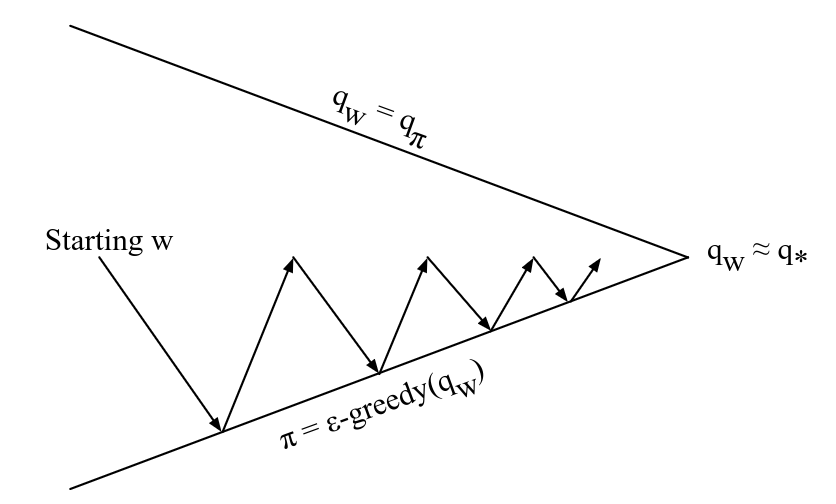
\includegraphics[width=0.5\textwidth]{figures/control_func_approx.png}
\end{figure}

As before we approximate the value function $\hat{q}(s,a,\mathbf{w}) \approx q_\pi(s,a)$ and minimize the MSE between approximate action-value function and true value action-value function:
\[
    J(\mathbf{w}) = \mathbb{E}\left[ (q_\pi(s,a) - \hat{q}(s,a,\mathbf{w}))^2 \right]
\]
And we use SGD to find a local minimum:

\begin{align*}
    -\frac{1}{2} \nabla_{\mathbf{w}} J(\mathbf{w}) &= \left( q_\pi(s,a) - \hat{q}(s,a,\mathbf{w}) \right) \nabla_{\mathbf{w}} \hat{q}(s,a,\mathbf{w}) \\
    \Delta \mathbf{w} &= \alpha \left( q_\pi(s,a) - \hat{q}(s,a,\mathbf{w}) \right) \nabla_{\mathbf{w}} \hat{q}(s,a,\mathbf{w})
\end{align*}

In general when dealing with continuous variables we cannot make a lookup table out of it since there are infinitely many states to deal with! So two possible solutions used in RL are the followings:
\begin{itemize}
    \item \textbf{Coarse Coding:} represents continuous states as binary features using overlapping circles, turning on features whenever a state falls inside them. Each cirle represents a single binary feature $x_i(s)$:
    \begin{itemize}
        \item If state $s$ lies in circle $i$ then $x_i(s) = 1$
        \item Else $x_i(s) = 0$
    \end{itemize}
    When a state $s$ is updated, the weights corresponding to all active circles update together. Any nearby state $s'$ that falls into the same overlapping circles instantly inherits that update-creating automatic, localized generalization.
    \item \textbf{Tile Coding:} is a fast, structured form of coarse coding that uses multiple uniform grid layers ("tilings") shifted slightly relative to each other, allowing linear models to generalize smoothly across continuous spaces.
\end{itemize}

\paragraph{Example: Mountain Car with Linear SARSA.}
The Mountain Car problem is a continuous control task where an underpowered car must reach a goal located at the top of a steep mountain slope on the right. Because gravity is stronger than the car's engine, applying full throttle from the valley is not enough to drive straight up the incline. To succeed, the agent must first take a counterintuitive action: driving in the opposite direction up the left slope to gather momentum, then using that built-up inertia along with full throttle to carry the car all the way up to the goal.

Here the reward is always $-1$ on all time steps until the car moves past the goal's position.

The feature vectors $\mathbf{x}(s,a)$ are created by tile coding and are then combined linearly with the parameter vector to approximate the action-value function.

\begin{figure}[htbp]
    \centering
    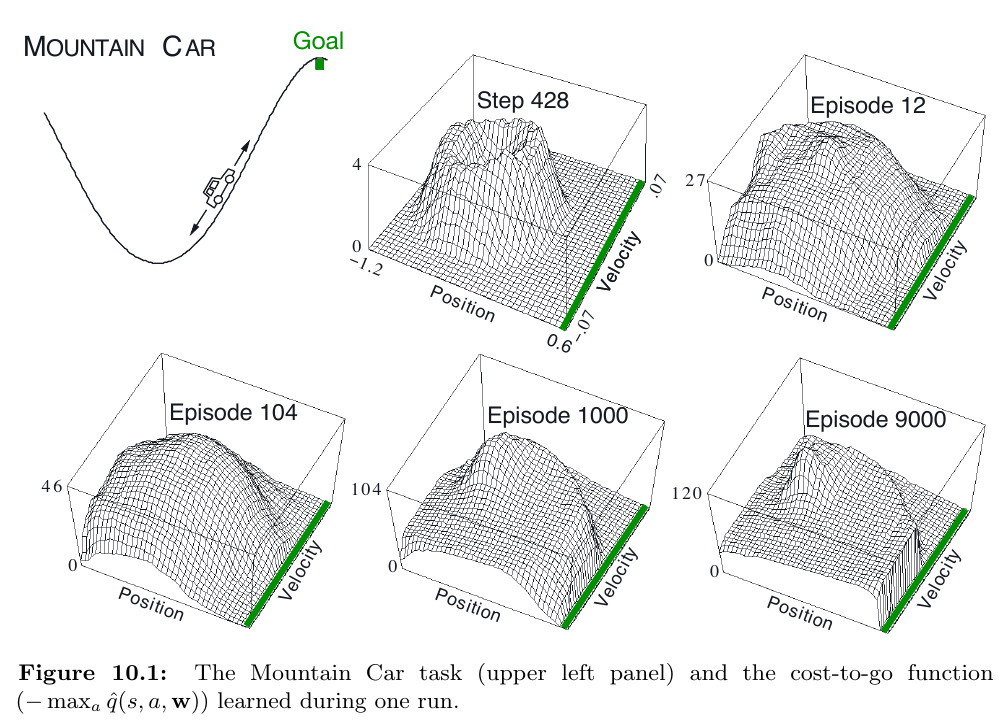
\includegraphics[width=0.5\textwidth]{figures/linear_sarsa_mountain_car.png}
\end{figure}

Shown is the negative of the value function (the \emph{cost- to-go} function) learned on a single run. The initial action values were all zero, which was optimistic (all true values are negative in this task), causing extensive exploration to occur even though the exploration parameter, $\varepsilon$, was 0. This can be seen in the middle-top panel of the figure, labeled “Step 428”. At this time not even one episode had been completed, but the car has oscillated back and forth in the valley, following circular trajectories in
state space. All the states visited frequently are valued worse than unexplored states, because the actual rewards have been worse than what was (unrealistically) expected. This continually drives the agent away from wherever it has been, to explore new states, until a solution is found.

\subsection{Algorithms Convergence}

\paragraph{Monte Carlo} With linear functions (and suitably decaying step sizes), MC converges to:
\begin{align*}
    \mathbf{w}_{\text{MC}} 
    &= \argmin_{\mathbf{w}} \mathbb{E}_\pi \!\left[ \left(G_t - v(S_t, \mathbf{w})\right)^2 \right] \\
    &= \argmin_{\mathbf{w}} \mathbb{E}_\pi \!\left[ \left(G_t - \mathbf{w}^\top \mathbf{x}_t\right)^2 \right] && \text{(using } v(S_t, \mathbf{w}) = \mathbf{w}^\top \mathbf{x}_t \text{)} \\
    &= \left( \mathbb{E}\left[ \mathbf{x}_t \mathbf{x}_t^\top \right] \right)^{-1} \mathbb{E}\left[ G_t \mathbf{x}_t \right]
\end{align*}

\paragraph{TD} With linear functions, TD converges to:
\[
    \mathbf{w}_{\text{TD}} = \left( \mathbb{E}\left[ \mathbf{x}_t \left(\mathbf{x}_t - \gamma \mathbf{x}_{t+1}\right)^\top \right] \right)^{-1} \mathbb{E}\left[ R_{t+1}\mathbf{x}_t \right]
\]

The TD update is not an actual \emph{gradient} update, but more of a \textbf{stochastic approximation} update (broader class than SGD):

\[
    \mathbf{w} \gets \mathbf{w} + \alpha ( \underbrace{R_{t+1} + \gamma \hat{v}(S_{t+1}, \mathbf{w})}_{\text{TD Target}} - \hat{v}(S_t, \mathbf{w}) ) \nabla_{\mathbf{w}} \hat{v}(S_t, \mathbf{w})
\]

It is not an actual gradient because, if we took the real gradient, we would get the following result:
$$\left( R_{t+1} + \gamma \hat{v}(S_{t+1}, \mathbf{w}) - \hat{v}(S_t, \mathbf{w}) \right) \left[ \mathbf{\color{red}{\gamma \nabla_{\mathbf{w}} \hat{v}(S_{t+1}, \mathbf{w})}} - \nabla_{\mathbf{w}} \hat{v}(S_t, \mathbf{w}) \right]$$

TD completely ignores the derivative of the target term ($\mathbf{\color{red}{\gamma \nabla_{\mathbf{w}} \hat{v}(S_{t+1}, \mathbf{w})}}$). It treats the TD target as if it was not dependent on $\mathbf{w}$: it takes into account the effect of changing the weight vector $\mathbf{w}$ on the estimate, but ignore its effect on the target. Because it only takes into account the effect of changing $\mathbf{w}$ on the estimate $\hat{v}(S_t, \mathbf{w})$, but ignores its effect on the target $\hat{v}(S_{t+1}, \mathbf{w})$, it is called a \emph{semi-gradient} method.

Because of this approximation TD does \textbf{not always converge}. When learning is on-policy with linear function approximation, the semi-gradient TD update happens to be stable because the stationary state distribution bounds the updates; however when we combine all three elements of the so-called \textbf{deadly triad}:
\begin{itemize}
    \item \textbf{Function Approximation:} scalable way of generalizing from a state space
    much larger than the memory and computational resources
    \item \textbf{Bootstrapping:} update targets that include existing estimates,  rather than relying exclusively on actual rewards and
    complete returns
    \item \textbf{Off-policy training:} training on a distribution of transitions other than that produced
    by the target policy. 
\end{itemize}

When $\mathbf{A}$ is not positive-definite, the semi-gradient update acts like an amplification feedback loop: updating $\mathbf{w}$ pushes the target $\hat{v}(S_{t+1}, \mathbf{w})$ even further away, causing the weight vector $\mathbf{w}$ to grow exponentially and diverge to $\pm \infty$.

Here $\mathbf{A} \coloneqq \mathbb{E}\big[\mathbf{x}_t(\mathbf{x}_t - \gamma \mathbf{x}_{t+1})^\top\big]$ is exactly the matrix inverted in the $\mathbf{w}_{TD}$ formula above: when it fails to be positive-definite, that inverse stops being a well-behaved contraction, which is the root cause of divergence.


\subsection{Batch Methods}
So far we have talked about gradient descent mechanisms: their updates are very simple, but they're not sample efficient. We see an experience once, we take an update adjusting the function approximation in the direction of that experience, and we move onto the next experience, throwing out the previous one: this is obviously not data-efficient. 

Batch method try to solve this issue by trying to find the best fitting value function to all the data we've seen in our batch (in this case, it's the agent's experience).

\subsubsection{Least Squares Temporal Difference (LSTD)}
The incremental TD updates from \ref{sec:incremental-methods} throw away each transition after a single small step. While this is memory-cheap it also is very sample-inefficient, and you also have to hand-tune a step size $\alpha$. LSTD's approach aims to solve directly for the $\mathbf{w}$ that best fits all the data you've collected, in one shot, with no step size to tune at all. The price is the $\mathcal{O}(n^2) - \mathcal{O}(n^3)$ cost per update instead of $\mathcal{O}(n)$, so it only makes sense when the feature dimension $d$ is small enough to afford it.

One way of finding this \emph{best fit} is to do it with the \emph{least squares} fit. Now if we want to fit our function approximator $\hat{v}(s, \mathbf{w}) \approx v_\pi(s)$ we can then define some dataset $\mathcal{D}$ consisting of $\langle \text{state}, \text{value}\rangle$ pairs:

\[
    \mathcal{D} = \{ \langle s_1, v_1^\pi \rangle, \langle s_2, v_2^\pi \rangle, \dots, \langle s_T v_T^\pi \rangle \}
\]

Assuming that the $v_i^\pi$ are some sort of oracle targets telling us the real value that $s_i$ should've had. Now which parameters \textbf{w} give the \emph{best fitting} value function $\hat{v}(s,\mathbf{w})$? \textbf{Least squares} algorithms find parameter vector \textbf{w} by minimizing the squared error between $\hat{v}(s_t, \mathbf{w})$ and target values $v_t^\pi$:

\begin{align*}
    \text{LS}(\mathbf{w}) &\doteq \sum_{t=1}^{T} (v_t^\pi - \hat{v}(s_t, \mathbf{w}))^2 \\
                          &= \mathbb{E}_{\mathcal{D}} [(v^\pi - \hat{v}(s,\mathbf{w}))^2]
\end{align*}

Now since $v_t^\pi$ is unknown, the best estimate for the value of state $s_t$ is the TD target:

\[
    R_{t+1} + \gamma \hat{v}(s_{t+1}, \mathbf{w})
\]

Recall that we already saw which parameters \textbf{w} gives us the best fitting for the value function:

\[
    \mathbf{w}_{\text{TD}} = \left( \mathbb{E}\left[ \mathbf{x}_t \left(\mathbf{x}_t - \gamma \mathbf{x}_{t+1}\right)^\top \right] \right)^{-1} \mathbb{E}\left[ R_{t+1}\mathbf{x}_t \right]
\]

So the idea is to use the closed-form equation's empirical loss:

\begin{align*}
    &\frac{1}{T} \sum_{t=1}^{T} \left( R_{t+1} + \gamma \hat{v}(s_{t+1}, \mathbf{w})  - \hat{v}(s_t, \mathbf{w}) \right) \mathbf{x}(s_t) \\
    &\Rightarrow \mathbf{w}_{\text{LSTD}} = \underbrace{\left( \sum_{t=1}^{T} \mathbf{x}(s_t) (\mathbf{x}(s_t) - \gamma \mathbf{x}(s_{t+1}))^\top \right)^{-1}}_{\mathbf{A}_t^{-1}} \underbrace{\left( \sum_{t=1}^{T} R_{t+1} \mathbf{x}(s_t) \right)}_{\mathbf{b}_t}
\end{align*}

We can update both $\mathbf{b}_t$ and $\mathbf{A}_t^{-1}$ incrementally online:
\begin{itemize}
    \item \textbf{Naive approach} ($\mathcal{O}(n^3)$):
    \[
        \mathbf{A}_{t+1} = \mathbf{A}_t + \mathbf{x}_t (\mathbf{x}_t - \gamma \mathbf{x}_{t+1})^\top \qquad \mathbf{b}_{t+1} = \mathbf{b}_t + R_{t+1} \mathbf{x}_t
    \]

    \item \textbf{Faster approach} ($\mathcal{O}(n^2)$):
    \begin{align*}
        \mathbf{A}_{t}^{-1} &= \mathbf{A}_{t-1}^{-1} - \frac{\mathbf{A}_{t-1}^{-1} \mathbf{x}_{t-1} (\mathbf{x}_{t-1} - \gamma \mathbf{x}_{t})^\top \mathbf{A}_{t-1}^{-1}}{1 + (\mathbf{x}_{t-1} - \gamma \mathbf{x}_{t})^\top \mathbf{A}_{t-1}^{-1} \mathbf{x}_{t-1}} \\
        \mathbf{b}_{t+1} &= \mathbf{b}_t + R_{t+1} \mathbf{x}_{t+1}
    \end{align*}
\end{itemize}

Where $\mathbf{x}_t \equiv \mathbf{x}(s_t)$.

\subsubsection{Experience Replay}
Here we make the dataset $\mathcal{D}$ an explicitly stored object (a replay buffer) containing past transitions $\langle S_t, A_t, R_t, S_{t+1} \rangle$. All we have to do now is sample transitions from this dataset $\langle S_t, A_t, R_t, S_{t+1} \rangle \sim \mathcal{D}$ and apply the semi-gradient update to $\mathbf{w}$ using the bootstrapped target $R_{t+1} + \gamma \hat{v}(S_{t+1}, \mathbf{w})$:

Here we make the dataset $\mathcal{D}$ an explicitly stored object (a replay buffer) containing past transitions $\langle S_t, A_t, R_t, S_{t+1} \rangle$. All we have to do now is sample transitions from this dataset $\langle S_t, A_t, R_t, S_{t+1} \rangle \sim \mathcal{D}$ and apply the semi-gradient update to $\mathbf{w}$ using the bootstrapped target $R_{t+1} + \gamma \hat{v}(S_{t+1}, \mathbf{w})$:

\[
    \Delta \mathbf{w} = \alpha \left( R_{t+1} + \gamma \hat{v}(S_{t+1}, \mathbf{w}) - \hat{v}(S_t, \mathbf{w}) \right) \nabla_{\mathbf{w}} \hat{v}(S_t, \mathbf{w})
\]

This converges to the least squares solution $\mathbf{w}^\pi = \argmin_\mathbf{w} \text{LS}(\mathbf{w})$